%&<latex>
\chapter{$\alpha$-DISK MODEL FITTING}
\label{chap:alpha_model_fitting}
\thispagestyle{empty}
\mquote{I'm your density.}{George McFly}

In this relatively short Chapter, we use the results of undisturbed SIM runs presented in Chapter~\ref{chap:cv_models} to obtain the free parameter $\alpha$ of Shakura-Sunyaev's $\alpha$-disc model. To do that, we utilize the area density solution in the Shakura-Sunyaev solution set \eqref{eq:alpha_model_solution}, for which we will find the best $\alpha$ parameter fit for SIM cases C2, C3, and C5.

\section{Fitting the area density distribution}
    The Shakura-Sunyaev $\alpha$-disc solution for the area density profile is

    \begin{equation}
        \Sigma = 5.2 \alpha^{-4/5} \dot{M}^{7/10}_{16} m^{1/4}_1 R^{-3/4}_{10} f^{14/5}\ \si{\gram\ \cm^{-2}},
        \label{eq:density_analytical}
    \end{equation}

    where we will threat the $\dot{M}_{16}$ and $m_1$ values as constats, and the boundary layer function $f$ will have the radius $R_*$ fixed to the value of inner radius of the disc $r_{\mathrm{in}}$

    \begin{align}
        \begin{split}
            \dot{M}_{16} &= 0.01, \\
            m_1 &= 0.63 M_{\odot}, \\
            f &= \left[ 1 - \left( \frac{r_{\mathrm{in}}}{R} \right)^{1/2} \right]^{1/4}. \\
        \end{split}
    \end{align}

    Therefore, the only remaining variable to optimize the function \eqref{eq:density_analytical} for (i.e., the response variable) is the parameter $\alpha$, while the independent variable (i.e., the predictor) is the radius $R_{10}$. Figure~\ref{fig:plot_density_analytical} shows several examples of dependencies for equation~\eqref{eq:density_analytical} using different values of $\alpha$ parameter.  
    
    The density data used for fitting we get from the SIM runs C2, C4, and C5 by transforming the individual cell masses into densities with the use of the known surface area of the disc's cells. The second step is to calculate the mean area density $\bar{\Sigma}(R_{10})$ by averaging the cell's densities ring-wise and also over several hundred simulation steps ($200$ steps, in this case, to be precise). 

    \begin{figure}[H]
    \begin{center}
        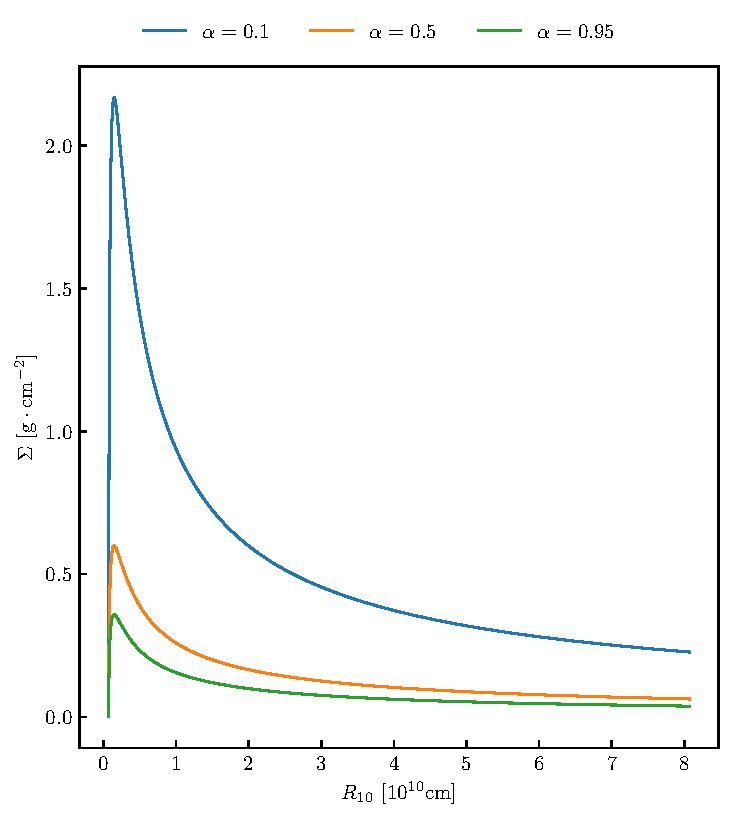
\includegraphics[width=1.0\textwidth]{img/plot_density_analytical.pdf}
    \end{center}
    \caption{Examples of Shakura-Sunyaev analytical area density solution.}
    \label{fig:plot_density_analytical}
    \end{figure}

    Figure~\ref{fig:plot_mean_density_fit} shows the Shakura-Sunyaev $\alpha$-disc area density $\Sigma$ solution~\eqref{eq:density_analytical} fited to mean area density data $\bar{\Sigma}$ extracted from C2, C3, and C4 SIM runs, respectivelly. The edge data (i.e., the inner and outer edge of the disc) were omitted from the fit because the irregular local conditions squee these data points. The outer edge's temperature and mass content are mostly a product of steady mass influx from the secondary component. To ensure numerical stability, the inner edge often triggers the low-value mass cut-off (see equation~\eqref{eq:m_cut_off}). 

    We can see that the MSH model produces a distribution that closely agrees with the analytical $\alpha$-disc solution. Therefore we can reliably obtain the value of the $\alpha$ parameter for specific MDH configurations. The particular value of $\alpha$ alpha could then be used to compute the distribution of other variables in the Shakura-Sunyaev solution set (see. equations~\eqref{eq:alpha_model_solution}).  
    
    \begin{figure}[H]
    \begin{center}
    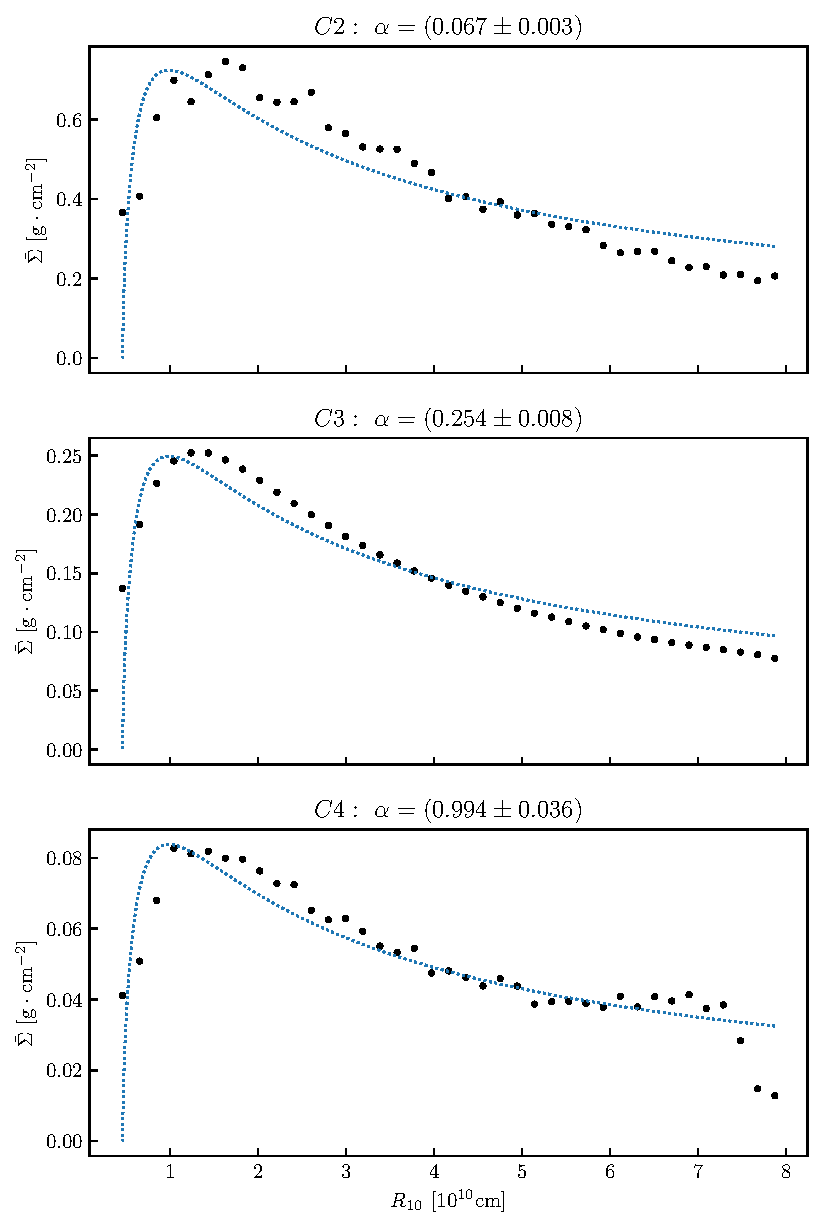
\includegraphics{img/plot_mean_density_fit.pdf}
    \end{center}
        \caption{Shakura-Sunyaev $\alpha$-parameter fits (dotted blue curves) for mean area density $\bar{\Sigma}$ extracted from C2 ($q=0.1, \psi=0.9$), C3 ($q=0.9, \psi=0.1$), and C4 ($q=0.9, \psi=0.9$) SIM runs. }
    \label{fig:plot_mean_density_fit}
    \end{figure}
